\documentclass[conference]{IEEEtran}
\IEEEoverridecommandlockouts

\usepackage{cite}
\usepackage{amsmath,amssymb,amsfonts}
\usepackage{algorithmic}
\usepackage{graphicx}
\usepackage{textcomp}
\usepackage{xcolor}
\usepackage{url}
\def\BibTeX{{\rm B\kern-.05em{\sc i\kern-.025em b}\kern-.08em
    T\kern-.1667em\lower.7ex\hbox{E}\kern-.125emX}}

\begin{document}

\title{Integrated Dataset Generation and Testing Platform for Dynamic Graph Neural Network ETA Prediction}

\author{\IEEEauthorblockN{Guy Tordjman}
\IEEEauthorblockA{\textit{Department of Mathematics and Computer Science} \\
\textit{The Open University}\\
University Road 1, Ra'anana, Israel \\
Email: turgibot@gmail.com}
\and
\IEEEauthorblockN{Nadav Voloch}
\IEEEauthorblockA{\textit{Department of Computer Engineering} \\
\textit{Ruppin Academic Center}\\
Emek Hefer, Israel \\
Email: nadavv@ruppin.ac.il}
}

\maketitle

\begin{abstract}
This paper presents an integrated platform combining Traffic-DSTG-Gen dataset generator and TrafficLab testing environment for Dynamic GNN ETA prediction. The system generates route-aware dynamic graphs from SUMO simulations and provides comprehensive real-time model evaluation capabilities for smart transportation research applications.
\end{abstract}

\begin{IEEEkeywords}
Graph Neural Networks, ETA Prediction, SUMO Simulation, Dataset Generation, Route-Aware Graphs, Testing Platform
\end{IEEEkeywords}

\section{Introduction}

Accurate Estimated Time of Arrival (ETA) prediction is crucial for modern transportation systems, enabling better route planning, traffic management, and improved navigation services. Dynamic Graph Neural Networks (GNNs) have emerged as powerful tools for modeling complex traffic networks with evolving topology and temporal dependencies.

However, developing and evaluating ETA prediction models presents significant challenges in dataset quality and feature richness. Traditional datasets rely on static sensors \cite{b1} or trajectory-based approaches \cite{b2}, which are limited in the number of features they can capture and often lack the comprehensive spatial-temporal information needed for accurate ETA prediction. Modern mobile technology and navigation applications can generate much richer datasets with detailed vehicle behavior, route information, and real-time traffic conditions. This gap necessitates the creation of simulation-based datasets that can capture the full complexity of traffic dynamics with rich feature sets, enabling more sophisticated model development and evaluation.

This work builds upon previous research in traffic prediction and ETA modeling \cite{b11,b12}, introducing an integrated system combining two complementary components: (1) Traffic-DSTG-Gen \cite{b3}, a dataset generator that creates route-aware dynamic spatio-temporal graphs from SUMO \cite{b4} traffic simulations, and (2) TrafficLab \cite{b5}, a real-time testing environment for model evaluation and deployment. The system addresses the critical need for both high-quality training data and robust testing environments for ETA prediction research.

\section{System Architecture and Methodology}

The integrated system consists of two main components working in tandem:

\textbf{Traffic-DSTG-Gen Dataset Generator:} This component generates route-aware dynamic spatio-temporal graphs from SUMO traffic simulations. The novel approach introduces a unique dataset structure where dynamic nodes represent vehicles and dynamic edges capture junction-vehicle-vehicle-junction relations, as illustrated in Fig. \ref{fig:graph_structure}:
\begin{itemize}
\item \textbf{Hybrid Node Structure:} Dynamic nodes represent vehicles, while static nodes represent junctions, enabling comprehensive traffic modeling
\item \textbf{Static-Dynamic Edge Architecture:} Static edges connect junctions (permanent road infrastructure), while dynamic edges capture real-time junction-vehicle-vehicle-junction relations that evolve with each snapshot
\item \textbf{Route-Aware Graph Construction:} Creates graphs with explicit route information for each vehicle, enabling accurate ETA prediction
\item \textbf{Dynamic Node Features:} 28-dimensional feature vectors for vehicles and junctions including speed, position, route progress, and destination information
\item \textbf{Temporal Sequences:} Sequential snapshots for time-series modeling with configurable time windows
\end{itemize}

\textbf{TrafficLab Testing Environment:} This component provides real-time testing capabilities for trained models:
\begin{itemize}
\item \textbf{Real-time Inference:} Live testing of ETA prediction models with actual traffic data
\item \textbf{Performance Benchmarking:} Comprehensive evaluation metrics including MAE, RMSE, and prediction reliability
\item \textbf{Interactive Visualization:} Real-time dashboard showing traffic conditions and model predictions
\end{itemize}

The system supports both offline batch processing for dataset generation and online real-time evaluation for model deployment, enabling researchers to develop, train, and test ETA prediction models in a unified environment.

\textbf{Dataset Generation Performance:} Traffic-DSTG-Gen successfully generates large-scale datasets with 80,000+ snapshots, supporting complex urban scenarios with multiple traffic zones. The system produces route-aware graphs with 28-dimensional node features and 7-dimensional edge features, enabling comprehensive ETA prediction research.

\textbf{Model Testing Capabilities:} TrafficLab enables real-time testing of various GNN architectures and provides users with comprehensive results and analysis for model evaluation and comparison, as exemplified by the MAE distribution across different trip durations (see Fig. \ref{fig:mae_plot}).

\textbf{Integrated Workflow:} The combined system supports end-to-end research workflows from dataset generation to model deployment, with seamless integration between SUMO simulation, graph construction, and real-time testing environments.

\begin{figure}[htbp]
\centerline{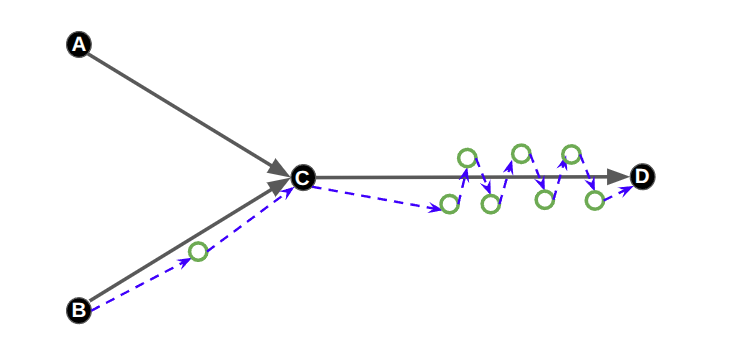
\includegraphics[width=0.5\textwidth]{nodes.png}}
\caption{Static and Dynamic Graph Structure: Black circles (A, B, C, D) represent static junction nodes, while green circles represent dynamic vehicle nodes. Solid gray edges connect static junctions, while dashed blue edges represent dynamic junction-vehicle-vehicle-junction relations that are created and updated on each snapshot.}
\label{fig:graph_structure}
\end{figure}

\begin{figure}[htbp]
\centerline{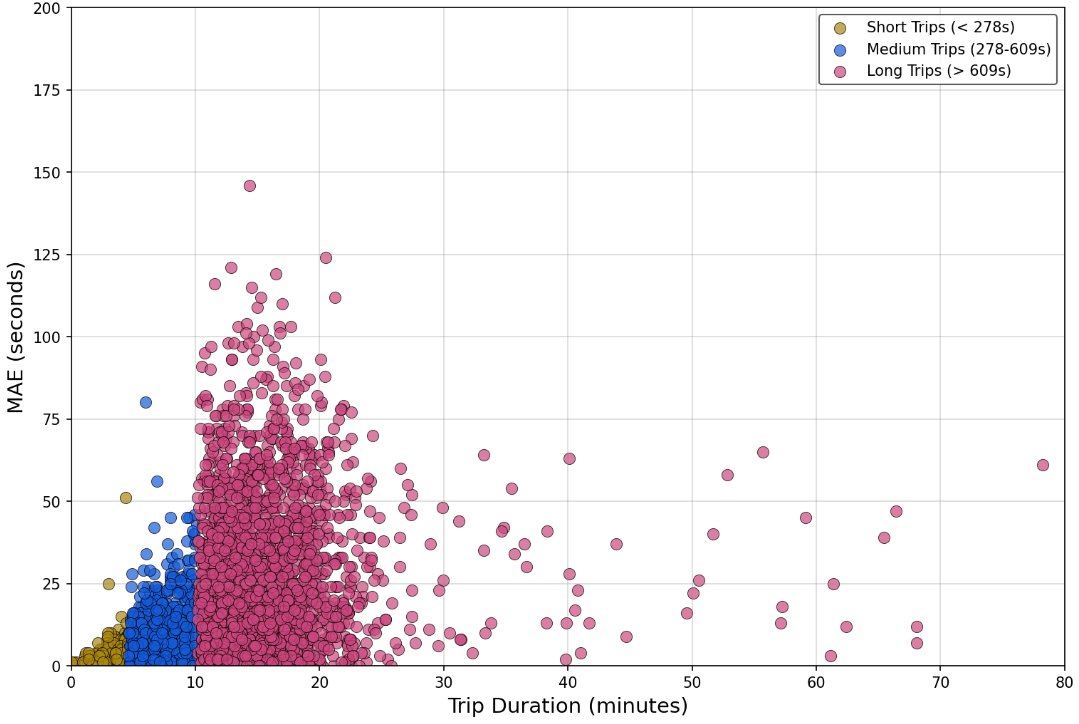
\includegraphics[width=0.5\textwidth]{mae_vs_time_plot_inverted.png}}
\caption{Mean Absolute Error (MAE) vs. Trip Duration showing performance across different trip categories. The plot demonstrates the platform's ability to evaluate model performance across varying trip durations, with short trips showing lower MAE values.}
\label{fig:mae_plot}
\end{figure}

\section{Conclusion}

This paper presents an integrated system combining Traffic-DSTG-Gen dataset generator and TrafficLab testing environment for Dynamic GNN ETA prediction research. The system addresses critical challenges in both dataset generation and model evaluation, providing researchers with comprehensive tools for developing and testing traffic prediction systems.

The integrated workflow from SUMO simulation to real-time model testing enables end-to-end research in ETA prediction, supporting the development of route-aware dynamic graph neural networks. Future work will focus on extending the platform to support federated learning scenarios and integrating additional traffic data sources.

Both components are available as open-source projects: Traffic-DSTG-Gen at \url{https://github.com/Ruppin-SmartTransportation/Traffic-DSTG-Gen} and TrafficLab at \url{https://github.com/Ruppin-SmartTransportation/TrafficLab}, providing a foundation for advancing ETA prediction technologies in smart transportation systems.

\section*{Acknowledgment}

The authors would like to thank Ruppin Academic center, Israel, and the Israeli Ministry of Innovation, Science and Technology (Proposal no. 0007846), for the continuing support in this research, implementation, and presentation. This study was funded by grant number 34836.

\begin{thebibliography}{00}
\bibitem{b1} J. J. Q. Yu, Y. Gu, H. Li, and S. Li, ``A survey on traffic prediction using big data,'' IEEE Trans. Intell. Transp. Syst., vol. 18, no. 10, pp. 2570-2586, 2017.
\bibitem{b2} H. Yao, X. Tang, H. Wei, G. Zheng, and Z. Li, ``Revisiting spatial-temporal similarity: A deep learning framework for traffic prediction,'' in Proc. 33rd AAAI Conf. Artif. Intell., 2019, pp. 5668-5675.
\bibitem{b3} Ruppin-SmartTransportation, ``Traffic-DSTG-Gen: Dynamic Spatio-Temporal Graph Generator for Traffic Simulation Data,'' 2024. [Online]. Available: \url{https://github.com/Ruppin-SmartTransportation/Traffic-DSTG-Gen}
\bibitem{b4} D. Krajzewicz, J. Erdmann, M. Behrisch, and L. Bieker, ``Recent development and applications of SUMO - Simulation of Urban MObility,'' Int. J. Adv. Syst. Meas., vol. 5, no. 3\&4, pp. 128-138, 2012.
\bibitem{b5} Ruppin-SmartTransportation, ``TrafficLab: Real-time Traffic Testing Environment,'' 2024. [Online]. Available: \url{https://demo.smart-transport.cloud/}
\bibitem{b6} Y. Li, R. Yu, C. Shahabi, and Y. Liu, ``Diffusion convolutional recurrent neural network: Data-driven traffic forecasting,'' in Proc. Int. Conf. Learn. Representations, 2018.
\bibitem{b7} B. Yu, H. Yin, and Z. Zhu, ``Spatio-temporal graph convolutional networks: A deep learning framework for traffic forecasting,'' in Proc. 27th Int. Joint Conf. Artif. Intell., 2018, pp. 3634-3640.
\bibitem{b8} J. Zhang, Y. Zheng, and D. Qi, ``Deep spatio-temporal residual networks for citywide crowd flows prediction,'' in Proc. 31st AAAI Conf. Artif. Intell., 2017, pp. 1655-1661.
\bibitem{b9} L. Bai, L. Yao, C. Li, X. Wang, and C. Wang, ``Adaptive graph convolutional recurrent network for traffic forecasting,'' in Proc. 34th Int. Conf. Neural Inf. Process. Syst., 2020, pp. 17804-17815.
\bibitem{b10} G. Jin, Y. Cui, L. Zeng, H. Tang, Y. Feng, J. Huang, and S. Ren, ``Traffic prediction based on spatial-temporal attention mechanism,'' in Proc. IEEE Int. Conf. Big Data, 2020, pp. 1746-1755.
\bibitem{b11} N. Voloch and N. Voloch-Bloch, ``Finding the Fastest Navigation Route by Real-Time Future Traffic Estimations,'' in Proc. IEEE Int. Conf. Microwaves, Communications, Antennas and Electronic Systems (COMCAS), 2021, pp. 1-6.
\bibitem{b12} N. Voloch, N. Penkar, and G. Tordjman, ``Estimating Accurate Traffic Time by Smart Simulative Route Predictions,'' in Proc. 24th IFIP Conf. e-Business, e-Services and e-Society (I3E), Limassol, Cyprus, 2025, pp. 1-8.
\end{thebibliography}

\end{document}
